\documentclass[logo,reportComp]{thesis}
\usepackage[cpp,pseudo]{mypackage}

\title{操作系统原理实验报告}
\subtitle{实验七:五状态进程模型}
\school{数据科学与计算机学院}
\author{陈鸿峥}
\classname{17大数据与人工智能}
\stunum{17341015}
\headercontext{操作系统原理实验报告}
% \authorremark{本实验报告用\LaTeX撰写,创建时间:\builddate\today}

\begin{document}

\maketitle

\section{实验目的}
\begin{itemize}
	\item 理解五状态进程模型的原理
	\item 实现更多的进程状态管理函数,如\verb'fork'、\verb'wait'、\verb'exit'等
	\item 能够将这些函数封装起来供上层应用程序使用
\end{itemize}

\section{实验要求}
% 实验目的和实验要求由老师提供实验项目文档中获取
在实验五或更后的原型基础上,进化你的原型操作系统,原型保留原有特征的基础上,设计满足下列要求的新原型操作系统:
\begin{enumerate}
	\item 实现控制的基本原语\verb'do_fork()'、\verb'do_wait()'、\verb'do_exit()'、\verb'blocked()'和\verb'wakeup()'
	\item 内核实现三系统调用\verb'fork()'、\verb'wait()'和\verb'exit()',并在C库中封装相关的系统调用
	\item 编写一个C语言程序,实现多进程合作的应用程序。
多进程合作的应用程序可以在下面的基础上完成:由父进程生成一个字符串,交给子进程统计其中字母的个数,然后在父进程中输出这一统计结果。
参考程序如下:
\begin{lstlisting}
char str[80] = "129djwqhdsajd128dw9i39ie93i8494urjoiew98kdkd";
int LetterNr = 0;

void CountLetter()
{
	int len = strlen(str);
	for(int i = 0; i < len; ++i)
		if(isalpha(str[i]))
			LetterNr++;
}

void main() {
	int pid = fork();
	if (pid == -1){
		printf("Error in fork!\n");
		return;
	}
	if (pid) {
		wait();
		printf("LetterNr = %d, I'm parent!\n", LetterNr);
	} else {
		CountLetter();
		printf("I'm child!\n");
		exit(0);
	}
	return;
}
\end{lstlisting}
编译连接你编写的用户程序,产生一个\verb'.com'文件,放进程原型操作系统映像盘中。
\end{enumerate}

\section{实验环境}
% 包括:硬件或虚拟机配置方法、软件工具与作用、方案的思想、相关原理、程序流程、算法和数据结构、程序关键模块,结合代码与程序中的位置进行解释。不得抄袭,否则按作弊处理。
% 实验方案包括相关基础原理、实验工具和环境、程序流程和算法思想、数据结构与程序模块功能说明,代码文档组成说明等
具体环境选择原因已在实验一报告中说明。
\begin{itemize}
	\item Windows 10系统 + Ubuntu 18.04(LTS)子系统
	\item gcc 7.3.0 + nasm 2.13.02 + GNU ld (Binutils) 2.3.0
	\item GNU Make 4.1
	\item Oracle VM VirtualBox 6.0.6
	\item Bochs 2.6.9
	\item Sublime Text 3 + Visual Studio Code 1.33.1
\end{itemize}

虚拟机配置:内存4M,1.44M虚拟软盘引导,1.44M虚拟硬盘。

\section{实验方案}
% 包括:主要工具安装使用过程及截图结果、程序过程中的操作步骤、测试数据、输入及输出说明、遇到的问题及解决情况、关键功能或操作的截图结果。不得抄袭,否则按作弊处理。
{\textbf{\textcolor{red}{本次实验继续沿用实验六保护模式的操作系统。}}}

本次实验亮点如下:
\begin{itemize}
	\item 增添了对\textbf{ELF文件}的读入、解析、执行
	\item 实现五状态进程模型,同时确保\textbf{不同特权级}的转换能够正常运行,且\textbf{不同进程空间、堆栈分配}不会重叠
	\item 增添\verb'fork'、\verb'wait'、\verb'exit'等系统调用(\textbf{内核态}),注意都能在\textbf{用户态程序}下调用
	\item 增添用户C程序的编译支持,增添\textbf{链接文件}\verb'link.ld'
	\item 支持\textbf{单用户程序多个fork及多个用户程序的进程管理}
\end{itemize}

\subsection{ELF文件}
可执行与可链接格式(Executable Linkable Format, ELF)是一种x86架构上类Unix操作系统的二进制文件标准格式,其具体内容可见图\ref{fig:elf}\footnote{图源自\url{https://www.cirosantilli.com/elf-hello-world/}}。
\begin{figure}[H]
\centering
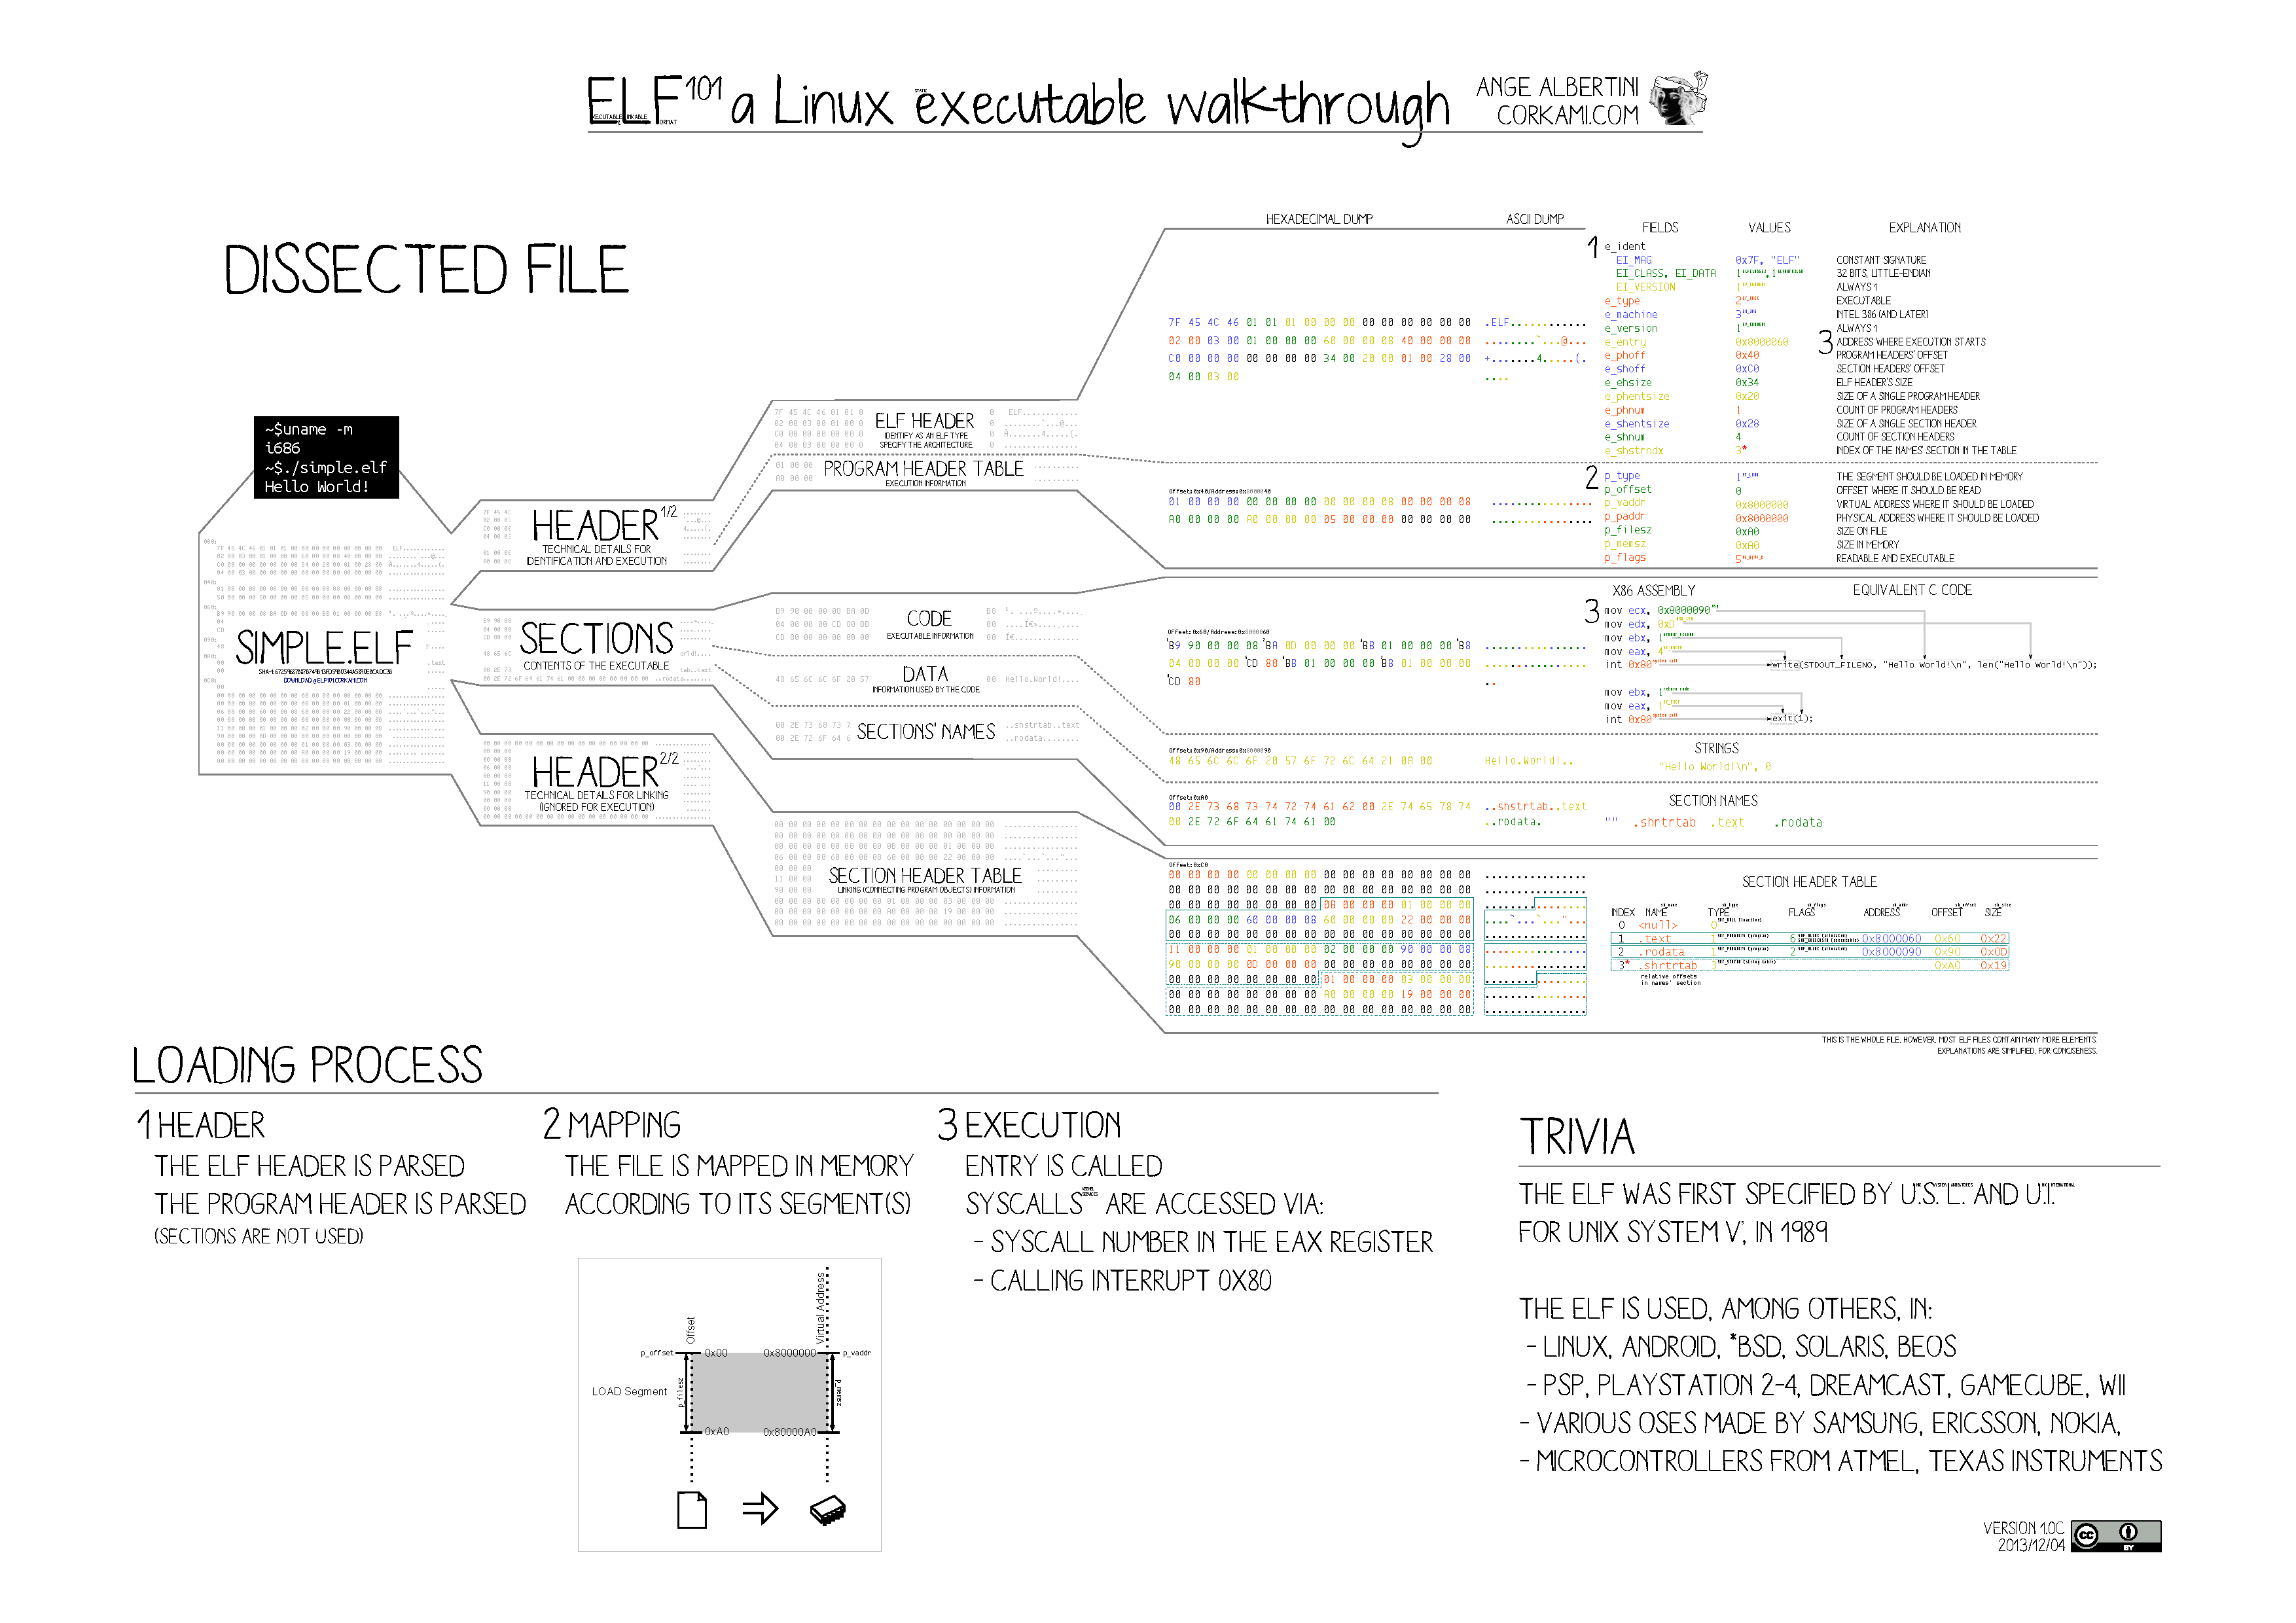
\includegraphics[width=\linewidth]{fig/elf101.pdf}
\caption{ELF格式说明}
\label{fig:elf}
\end{figure}

通过以下几条指令可以查看ELF文件的内容
\begin{lstlisting}[language=bash]
readelf -h fork_test.out ## show elf header
readelf -S fork_test.out ## show section headers
readelf -l fork_test.out ## show program headers
objdump -d fork_test.out ## show assembly
\end{lstlisting}

ELF文件由四个部分组成,分别是ELF头、程序头表、节和节头表四个部分组成。
其基本信息包含在\verb'elf.h'中,借鉴了清华UCore的格式定义,如下所示。
\begin{lstlisting}
/* file header */
typedef struct elfhdr {
    uint32_t e_magic;     // must equal ELF_MAGIC
    uint8_t  e_elf[12];
    uint16_t e_type;      // 1=relocatable, 2=executable, 3=shared object, 4=core image
    uint16_t e_machine;   // 3=x86, 4=68K, etc.
    uint32_t e_version;   // file version, always 1
    uint32_t e_entry;     // entry point if executable
    uint32_t e_phoff;     // file position of program header or 0
    uint32_t e_shoff;     // file position of section header or 0
    uint32_t e_flags;     // architecture-specific flags, usually 0
    uint16_t e_ehsize;    // size of this elf header
    uint16_t e_phentsize; // size of an entry in program header
    uint16_t e_phnum;     // number of entries in program header or 0
    uint16_t e_shentsize; // size of an entry in section header
    uint16_t e_shnum;     // number of entries in section header or 0
    uint16_t e_shstrndx;  // section number that contains section name strings
} elfhdr;

/* program section header */
typedef struct prghdr {
    uint32_t p_type;   // loadable code or data, dynamic linking info, etc.
    uint32_t p_offset; // file offset of segment
    uint32_t p_va;     // virtual address to map segment
    uint32_t p_pa;     // physical address
    uint32_t p_filesz; // size of segment in file
    uint32_t p_memsz;  // size of segment in memory (bigger if contains bss)
    uint32_t p_flags;  // read/write/execute bits
    uint32_t p_align;  // required alignment, invariably hardware page size
} prghdr;
\end{lstlisting}

其实我们需要关心的只有其中几项,包括
\begin{itemize}
	\item \verb'e_magic':是否为合法的ELF文件
	\item \verb'e_entry':可执行文件的入口,这里我通过链接文件\verb'link.ld'指定入口点为\verb'main'函数
	\item \verb'p_offset':程序段在ELF文件中的偏移量
	\item \verb'p_memsz':程序段的大小
\end{itemize}

故可以得到下面的ELF文件加载、执行逻辑(见\verb'user.h'文件),这一部分全部是\textcolor{red}{\textbf{原创内容}}。
一定要注意,ELF文件头是占空间的,故要先对文件头进行解析,然后再将后面实际程序的执行代码加载到内存中。
\begin{lstlisting}
oid exec_elf(int num) {
	disable();

	uintptr_t addr_exec = ADDR_USER_START+(num-1)*PROC_SIZE;
	uintptr_t addr = (uintptr_t)bin_img;

	read_sectors(addr,(num-1)*2,30);

	// parse elf header
	elfhdr eh;
	memcpy((void*)&eh,(void*)addr,sizeof(elfhdr));

	if (eh.e_magic != ELF_MAGIC){
		put_error("Bad elf file!");
		for(;;){}
	}

	// parse program header
	prghdr ph;
	for (int i = 0, offset = eh.e_phoff;
			i < eh.e_phnum; i++, offset += eh.e_phentsize){
		memcpy((void*)&ph,(void*)(addr+offset),eh.e_phentsize);
		if (i == 0)
			memcpy((void*)addr_exec,(void*)(addr+ph.p_offset),ph.p_memsz);
	}

	process* pp = proc_create(USER_CS,USER_DS,eh.e_entry);
	schedule_proc();
}
\end{lstlisting}
\begin{itemize}
	\item 首先将ELF文件读入到\verb'bin_img'中,这里预设程序大小为30个扇区
	\item 然后直接拷贝ELF头到结构体\verb'eh'中,由于顺序已经确定,故不需要对结构体元素一一赋值
	\item 通过\verb'ELF_MAGIC'判断ELF头是否合法,合法则再执行下面步骤
	\item 拷贝程序头到结构体\verb'ph'中,然后将\verb'[p_offset,p_offset+p_memsz]'实际程序的执行代码全部拷贝到进程空间中
	\item 创建进程入口地址为\verb'e_entry',然后开始进程调度执行
\end{itemize}

\subsection{五状态进程模型}
五状态进程模型我依照图\ref{fig:five-state}进行命名和定义。
\begin{figure}[H]
\centering
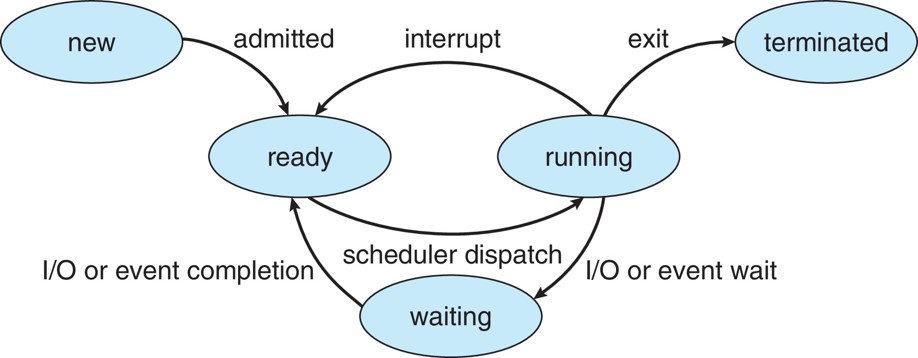
\includegraphics[width=0.5\linewidth]{fig/five-state.jpg}
\caption{五状态进程模型}
\label{fig:five-state}
\end{figure}

\subsubsection{fork}
这里一个关键问题在于保护模式下用户程序都处在\textbf{用户态}执行,而创建管理进程这些函数都属于\textbf{内核态}函数,如何ring 3的程序调用ring 0的例程这是需要考虑的。
而我的解决方案是通过\textbf{中断调用}的方式,需要满足以下两点。
\begin{itemize}
	\item 系统中断\verb'0x80'设置代码段为内核代码段,但特权级DPL为3
	\item 内核代码段与用户代码段重叠,在GDT中定义
\end{itemize}

用户C程序会包含\verb'api.h'的头文件,其中封装了用户态的\verb'fork'函数,如下所示,在C中内嵌汇编代码实现。

通过\verb'eax'寄存器传递功能号,然后调用系统中断\verb'0x80',进入内核态的\verb'do_fork'进行执行,然后返回用户态,再次利用\verb'eax'寄存器进行返回值传递。
\begin{lstlisting}
int fork() {
	int pid;
	asm volatile (
		"mov eax, 10\n\t"
		"int 0x80\n\t"
		:"=a"(pid):);
	return pid;
}
\end{lstlisting}

当调用了\verb'0x80'中断后,会跳转到\verb'sys_interrupt_handler'。
先关中断,然后立即对现场进行保护\verb'save_proc_entry'(这里逻辑与实验六切换进程第一步保存进程状态的逻辑相同,不再赘述),方便后续的\verb'fork'操作。
注意这里保存的是上述\verb'int 0x80'的下一条指令\verb'mov [pid], eax'的\verb'eip'值,这对父子进程的返回值有着至关重要的作用\footnote{保存现场不一定要在中断调用这里完成,我见到有些操作系统实现是在内核态的中断处理程序中直接读取eip创建新的进程的,然后通过当前进程是否是父进程判断返回什么值。这种情况下,fork出来的进程将处在内核态中,返回用户态程序还要切换堆栈非常麻烦。而采用我\textcolor{red}{\textbf{原创}}的这种方法则可以在fork出来后,依然在ring 3顺序执行用户态程序,且确保了父子进程的返回值不同。}。

由于C语言采用\verb'eax'存储返回值,故这里注意不要破坏现场,执行完中断处理程序后直接返回即可。
\begin{lstlisting}[language={[x86masm]Assembler}]
sys_interrupt_handler:
	cli
	jmp save_proc_entry
save_proc_entry_ret:
	push eax            ; Functional number
	call sys_interrupt_handler_main
	pop ebx             ; Remember to pop out
	; eax store the return value
	sti
	iretd
\end{lstlisting}

\verb'fork'的核心代码如下,除了要拷贝PCB外,核心关键点是还要\textbf{拷贝整个进程栈}。
否则父进程继续执行将会将原来堆栈的内容弹出,使得子进程无法再继续使用。

至于父子进程返回值不同的问题,前面脚注已经提及。
父进程直接返回子进程ID,而子进程通过修改\verb'regImg.eax'的值,使得进程切换后的\verb'eax'就是$0$。
\begin{lstlisting}
int do_fork() {

	disable();
	process* child;

	// find empty entry
	if ((child = proc_alloc()) == 0) {
		enable();
		return -1; // fail to create child process
	}

	// copy PCB, which has been saved by interrupt
	copy_PCB(child,curr_proc); // stack must be changed!

	// copy stack
	memcpy((void*)(child->regImg.user_esp),
		(void*)(curr_proc->regImg.user_esp),
		(curr_proc->regImg.ebp - curr_proc->regImg.user_esp)*2); // each entry 32-bit

	// set state
	child->regImg.eax = 0; // set child process return value
	child->parent = curr_proc;
	child->status = PROC_READY;
	reset_time(child);

	return child->pid;
}
\end{lstlisting}

\subsubsection{进程管理}
\verb'wait'逻辑很简单,就是切换进程状态,然后立即执行调度。
\begin{lstlisting}
void do_wait() {
	disable();
	curr_proc->status = PROC_WAITING;
	schedule_proc();
	enable();
}
\end{lstlisting}

同理\verb'exit'如下,需要唤醒父进程。
\begin{lstlisting}
void do_exit() {
	disable();
	curr_proc->status = PROC_TERMINATED;
	wakeup(curr_proc->parent->pid);
	enable();
}
\end{lstlisting}

\verb'wakeup'则找到父进程,然后将其状态更改回就绪,调用进程调度。
\begin{lstlisting}
void wakeup(uint8_t pid) {
	disable();
	for (process* pp = &proc_list[0]; pp < &proc_list[MAX_PROCESS]; ++pp){
		if (pp->pid == pid && pp->status == PROC_WAITING){
			pp->status = PROC_READY;
			schedule_proc();
			enable();
			return;
		}
	}
	enable();
}
\end{lstlisting}

调度模块相比起实验六做了一些改变,如下所示。
\begin{lstlisting}
process* proc_pick()
{
	int curr_index = -1;
	// find current running process
	for (int i = 0; i < MAX_PROCESS; ++i){
		if (proc_list[i].status == PROC_RUNNING){
			curr_index = i;
			break;
		}
	}
	// round-robin
	for (int i = 0; i < MAX_PROCESS; ++i){
		int index = (i + 1 + curr_index) % MAX_PROCESS;
		if (proc_list[index].status == PROC_READY)
			return &proc_list[index];
	}
	if (curr_index != -1) // no choice but the process still running
		return &proc_list[curr_index];
	else
		return NULL;
}

void schedule_proc()
{
	process* pp = proc_pick();
	if (pp == NULL)
		return;

	proc_switch(pp);
}
\end{lstlisting}

\subsubsection{系统调用}
目前关于进程的操作函数有以下这些(内核态),大部分都已在实验六中说明。
\begin{itemize}
	\item \verb'proc_init':初始化
	\item \verb'proc_alloc':分配新进程,状态由\verb'NEW'变更为\verb'READY'
	\item \verb'proc_create':根据地址创建新进程,结合\verb'alloc'一起使用
	\item \verb'proc_pick':挑选\verb'READY'进程
	\item \verb'save_proc':保存进程状态
	\item \verb'restart_proc':恢复进程状态
	\item \verb'proc_switch':进程切换
	\item \verb'schedule_proc':进程调度
	\item \verb'do_fork':进程分支
	\item \verb'do_wait'/\verb'blocked':进程等待/阻塞
	\item \verb'do_exit':(子)进程退出
	\item \verb'wakeup':进程唤醒
	\item \verb'sys_get_pid':返回进程ID
	\item \verb'kill':结束进程
\end{itemize}

目前的系统调用如表\ref{tab:syscall}所示,均可直接在用户态调用。
\begin{table}[H]
\caption{系统调用功能表}
\label{tab:syscall}
\centering
\begin{tabular}{|c|c|}\hline
\textbf{功能号} & \textbf{功能}\\\hline
0 & 输出OS Logo\\\hline
1 & 睡眠100ms\\\hline
10 & fork\\\hline
11 & wait\\\hline
12 & exit\\\hline
13 & get\_pid\\\hline
100 & 返回内核Shell\\\hline
\end{tabular}
\end{table}

\section{实验结果}
\begin{figure}[H]
\centering
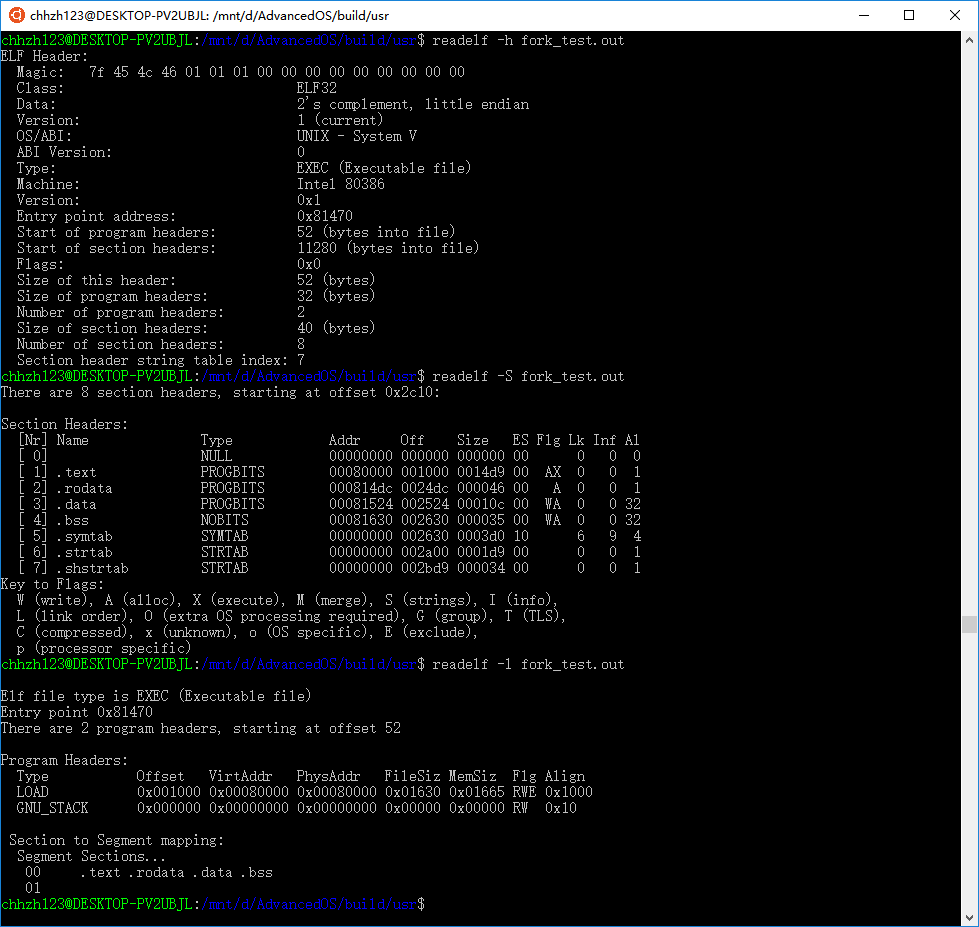
\includegraphics[width=0.8\linewidth]{fig/readelf.PNG}
\caption{利用readelf查看ELF文件内容}
\label{fig:readelf}
\end{figure}

参考程序已在老师程序的基础上进行了修改,见首页,分别输出父子进程,如图\ref{fig:fork}所示,\verb'exec 7'调用执行\verb'fork_test.c',结果为27。

同时,我也自己再写了一个测试程序\verb'fork2.c',如下,用于测试\textbf{多个子进程}环境下是否还能正常运行。
\begin{lstlisting}
#include "stdio.h"
#include "api.h"

void main()
{
	int a = fork();
	int b = fork();
	int c = fork();
	if (a == 0 || b == 0 || c == 0)
		printf("This is hello from process %d! (child)\n", get_pid());
	else
		printf("This is hello from process %d! (parent)\n", get_pid());
	return;
}
\end{lstlisting}

同样结果如图\ref{fig:fork}所示,由于\verb'fork2.c'没有\verb'wait'指令等待子进程完成,故会返回多次Shell。
抛出Shell命令,可以看出,结果产生8个进程是正确的。
\begin{figure}[H]
\centering
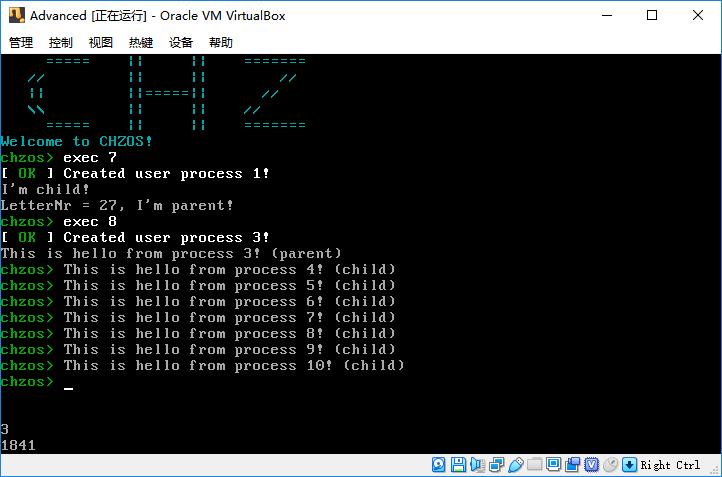
\includegraphics[width=0.8\linewidth]{fig/fork.PNG}
\caption{fork演示多进程合作}
\label{fig:fork}
\end{figure}

注意:
\begin{itemize}
	\item 这里的用户程序是用gcc编译为\textbf{ELF文件}存储入虚拟硬盘后,在OS内核执行过程中\textbf{动态载入、解析、执行}的
	\item 执行完用户程序(用户态)后将\textbf{返回内核Shell}(内核态)
	\item 这里的\verb'exec 7'和\verb'exec 8'都是在交互界面输入后才执行,不是预先安排好的。
	可以看出本套进程管理系统不仅对单个程序内部的多进程管理做得很好,而且对多个程序的进程管理也可以胜任。
\end{itemize}


\section{实验总结}
% 每人必需写一段,文字不少于500字,可以写心得体会、问题讨论与思考、新的设想、感言总结或提出建议等等。不得抄袭,否则按作弊处理。
一开始想着实验六已经将保护模式操作系统的整个框架搭建起来,继续做实验七应该很快。
但事实证明我又错了。
保护模式每一个实验都非常耗时,核心问题都在于\textbf{用户态和内核态}之间如何进行切换。

为了更好地管理用户程序,以及具有一定的普适性,这一次将ELF文件支持添加到我的操作系统中。
虽然ELF的格式较为简单,但要理解透彻并具体实施还是要考虑很多细节的。
比如最开始老是没想明白如何将核心用户程序段加载到对应位置,因为以往都有汇编作为入口,跳转地址就直接是汇编程序的第一行。
但现在程序不是一个扁平的二进制文件,编译出来有一大堆函数,入口点就不再是第一条指令了。
而ELF头正是给出了文件的这些信息,故需要先进行解析,然后再将后面的程序正文读到内存的指定位置,然后通过ELF头给出的入口地址直接跳转。
其实从这个角度看,ELF反而让用户程序好管理了很多。

\verb'fork'函数的编写也耗费了我很多脑细胞,因为没有采用常规思路,完全依照\verb'fork'函数要达成的功能自己想怎么实现。
关键在于怎么让\verb'fork'的父子进程返回不同的值,这一点深入了解了C函数调用的汇编原理就好做很多,核心就是通过\verb'eax'寄存器进行传递。
所以针对父进程可以直接返回子进程ID;而针对子进程,则在父进程中对子进程的\verb'eax'进行设置,切换进程时就会自动恢复。

现在我的操作系统最大的问题还在于用户程序的管理,每次添加一个用户程序,都要改一遍\verb'Makefile'文件,然后改一大批头文件(只要包含用户程序的都要进行修改),还要自己算内存地址,这些都是相当不智能的地方。
但之后继续往下做了分页和文件系统应该就更好管理。


\section{参考资料}
\begin{enumerate}
	\item OS Development Series, \url{http://www.brokenthorn.com/Resources/OSDevIndex.html}
	\item Roll your own toy UNIX-clone OS, \url{http://www.jamesmolloy.co.uk/tutorial_html/}
	\item The little book about OS development, \url{http://littleosbook.github.io/}
	\item Writing a Simple Operating System from Scratch, \url{http://www.cs.bham.ac.uk/~exr/lectures/opsys/10_11/lectures/os-dev.pdf}
	\item Intel$^{\textregistered}$ 64 and IA-32 Architectures Software Developer's Manual
	\item UCore OS Lab, \url{https://github.com/chyyuu/ucore_os_lab}
	\item CMU CS 15-410, Operating System Design and Implementation, \url{https://www.cs.cmu.edu/~410/}
	\item 李忠,王晓波,余洁,《x86汇编语言-从实模式到保护模式》,电子工业出版社,2013
	\item ELF Hello World Tutorial, \url{https://www.cirosantilli.com/elf-hello-world/}
\end{enumerate}

\appendix
\appendixconfig
\section{程序清单}
\subsection{内核核心代码}
\begin{center}
\begin{tabular}{|c|l|l|}\hline
\textbf{序号} & \textbf{文件} & \textbf{描述} \\\hline
1 & \verb'bootloader.asm' & 主引导程序\\\hline
2 & \verb'kernel_entry.asm' & 内核汇编入口程序\\\hline
3 & \verb'kernel.c' & 内核C入口程序\\\hline
4 & \verb'Makefile' & 自动编译指令文件\\\hline
5 & \verb'bootflpy.img' & 引导程序/内核软盘\\\hline
6 & \verb'mydisk.hdd' & 虚拟硬盘\\\hline
7 & \verb'bochsrc.bxrc' & Bochs配置文件\\\hline
\end{tabular}
\end{center}

\subsection{内核头文件}
\begin{center}
\begin{tabular}{|c|l|l|}\hline
\textbf{序号} & \textbf{文件} & \textbf{描述} \\\hline
1 & \verb'disk_load.inc' & BIOS读取磁盘\\\hline
2 & \verb'show.inc' & 常用汇编字符显示\\\hline
3 & \verb'gdt.inc' & 汇编全局描述符表\\\hline
4 & \verb'gdt.h' & C全局描述符表\\\hline
5 & \verb'idt.h' & 中断描述符表\\\hline
6 & \verb'hal.h' & 硬件抽象层\\\hline
6.1 & \verb'pic.h' & 可编程中断控制器\\\hline
6.2 & \verb'pit.h' & 可编程区间计时器\\\hline
6.3 & \verb'keyboard.h' & 键盘处理\\\hline
6.4 & \verb'tss.h' & 任务状态段\\\hline
6.5 & \verb'ide.h' & 硬盘读取\\\hline
7 & \verb'io.h' & I/O编程\\\hline
8 & \verb'exception.h' & 异常处理\\\hline
9 & \verb'syscall.h' & 系统调用\\\hline
10 & \verb'task.h' & 多进程设施\\\hline
11 & \verb'user.h' & 用户程序处理\\\hline
12 & \verb'terminal.h' & Shell\\\hline
13 & \verb'scancode.h' & 扫描码\\\hline
14 & \verb'stdio.h' & 标准输入输出\\\hline
15 & \verb'string.h' & 字符串处理\\\hline
16 & \verb'elf.h' & ELF文件处理\\\hline
17 & \verb'api.h' & 进程管理API\\\hline
\end{tabular}
\end{center}

\subsection{用户程序}
用户程序都放置在\verb'usr'文件夹中。
\begin{center}
\begin{tabular}{|c|l|l|}\hline
\textbf{序号} & \textbf{文件} & \textbf{描述} \\\hline
1-4 & \verb'prgX.asm' & 飞翔字符用户程序\\\hline
5 & \verb'box.asm' & 画框用户程序\\\hline
6 & \verb'sys_test.asm' & 系统中断测试\\\hline
7 & \verb'fork_test.c' & 进程分支测试\\\hline
8 & \verb'fork2.c' & 进程多分支测试\\\hline
\end{tabular}
\end{center}

\end{document}

% 实验提交内容
% 实验报告:电子版(Word2003的DOC格式或PDF格式)
% 原程序文件及可执行代码程序文件
% 测试输入数据文件和输出数据文件
% 虚拟机软盘映像文件

% 基础实验项目5个和扩展实验7个
% 实验项目,迟交影响成绩评价!
% 工具与环境可由选择,开发新型工具或优化一套开发环境都可加分!
% 一系列基础实验项目必须连续完成,当前项目只能在前一个项目的基础上进行,体现出前后的进化关系,否则要被约谈,证明没有抄袭行为!
% 一个项目可提交多个改进的版本,实现新功能和个性化特征都有利于提高相应项目的成绩。
% 实验项目提交内容用winrar工具整体压缩打包,统一格式命名为:
%	<学号>+<姓名>+<实验项目号>+<版本号>.rar
%	姓名(学号)实验NvX.zip
%	实验报告、项目文件夹、映像文件
%	ftp://172.18.216.232 sysuac 下周六23:59

% 免考
% 条件:实验1~6全部评价AAAAB+B+或相当
% 最终成绩可能范围:75分以上